\section{Results}

This section reports on the study of 399 MAPMTs H12700, acquired for the RICH2 detector upgrade. All of them were tested in the same conditions by the groups of six mounted in the Maroc tiles and irradiated simultaneously. The test procedure included six different setup conditions: two sets of the high voltage applied (1000 V and 1100 V), and three laser light intensity settings at the wheel positions 3, 4, and 6. The data were accumulated and pre-processed to make the non-linearity corrections and to convert the amplitudes to the units of electric charge. After that the data were transferred to the ``parameterization factory'' computer workstation in which every accumulated spectrum was automatically analyzed and approximated with the 12-parameter fitting function, as it is explained in the earlier sections. Every PMT was issued the ``MAPMT passport'' document listing the fit parameters for every measurement, for all 64 anodes, showing the extracted SPE functions, and the parameter dependencies on pixel number, as illustrated in Figs. \ref{fig:LA2527_passport} and \ref{fig:LA2527_passport_spectra}. The most important parameters extracted from the analysis for every pixel are $scale$, measuring the average charge collected at the anode from the single photoelectron events; the average multiplicity $\mu$ of the photoelectrons per laser pulse, that can be converted to the quantum efficiency of the pixel when normalized to calibrated incoming light in the pulse; the calculated optimal threshold value for the separation of the single photoelectron events from pedestal (including the cross talk background), and corresponding estimate of the photodetection efficiency based on that value. Parameters of interest are also the characteristics of the photomultiplier, such as the evaluated in the model gain on the first dynode, amplitude width and intensity of the cross talk signal. The pedestal $\sigma$ parameter characterizes the quality of the Maroc measurement channel.

The six independent measurements in different conditions were used to verify the self-consistency of the results, using the model approximation features allowing the $scale$ parameter to be measured at various light conditions, ideally providing the same value, and similarly allowing the $\mu$ parameter (and hence the quantum efficiency) to be measured at various high voltages, also providing the same value. These features may be found in all ``MAPMT passports'', and also they are further illustrated in the following figures. Fig. \ref{fig:pglobal_sc} shows the distribution of $scale$ parameter through the whole data set, separately for different high voltages and illumination settings. The distributions are clearly identical if obtained in different illuminations, and the change in high voltage is seen as approximate multiplication of the $scale$ parameter by a factor about 2 when switching from HV = 1000 V to HV = 1100 V. Logarithmic scale in x axis in the plot helps to see the multiplication as a shift on the plot, roughly preserving the shape of the distribution. 
\begin{figure}[hbt]
	\centering
	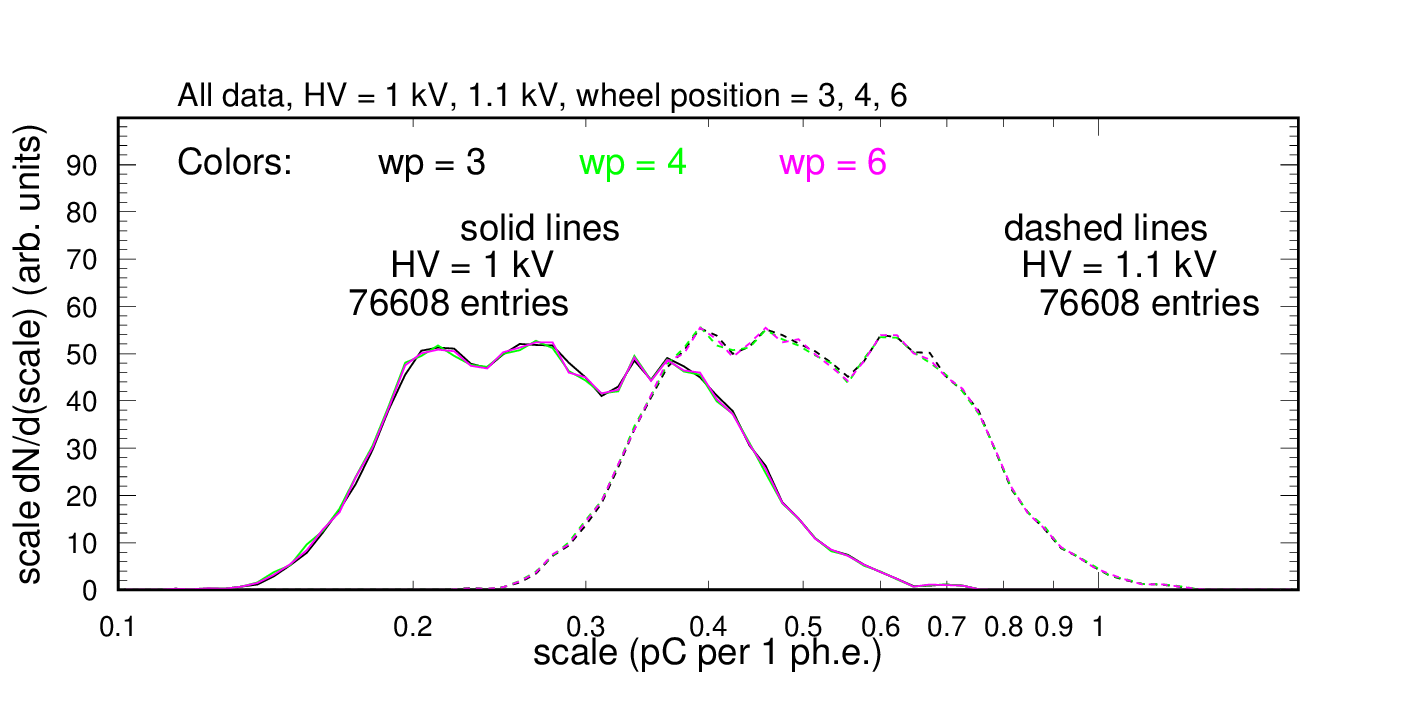
\includegraphics[width=0.98\linewidth,trim=0 15 50 35,clip]{figures/pglobal_sc.pdf}
	\caption{Distribution of $scale$ (average charge per ph.e) as determined by the fitting procedure for a set of 399 PMTs. All measured pixels contributed to the plots. Distributions measured at HV = 1000 V are shown by solid lines, the ones at HV = 1100 V by dashed lines. The three colors correspond to the three different illuminations (essentially on top of each other).
	}
	\label{fig:pglobal_sc}
\end{figure}

The stability and consistency of the fitting procedure is illustrated in Fig. \ref{fig:pglobal_Rs} in which every measured $scale$ parameter is normalized to the value of $scale$ averaged over the three measurements on the same pixel at the three different illuminations. The value of the ratio $R_{\mathrm{s}}$ serves as an estimate of the statistical error of the $scale$ evaluation procedure, and is approximately within 0.75\% for the tests at HV = 1.0 kV, and within 0.5\% at HV = 1.1 kV 
\begin{figure}[hbt]
	\centering
	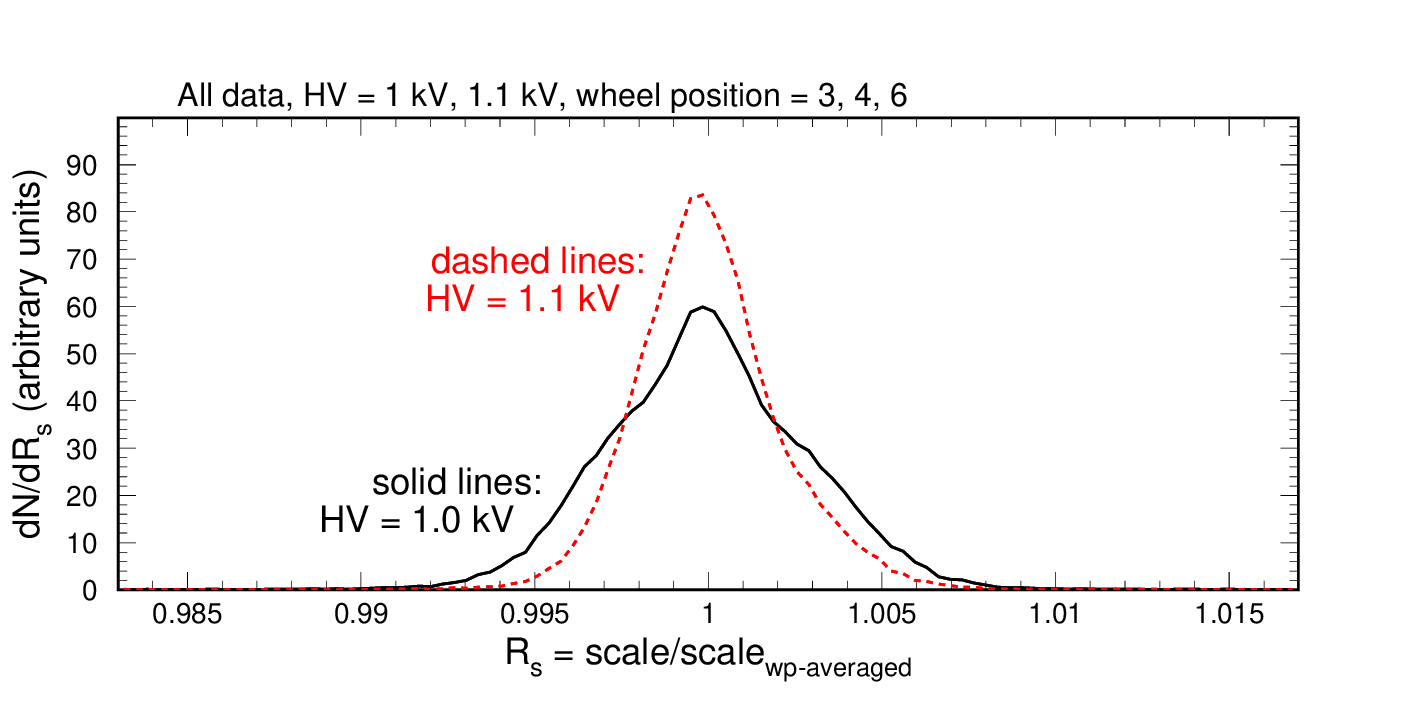
\includegraphics[width=0.98\linewidth, trim=0 15 50 35, clip]{figures/pglobal_Rs.pdf}
	\caption{Parameter $scale$ normalized to its average value over the three different illumination settings (wheel positions 3, 4, and 6).}
	\label{fig:pglobal_Rs}
\end{figure}

In the bulk measurements one PMT was measured in one Maroc location. To be confident that different Maroc locations do not systematically contribute to the differences between the PMTs we compared all six locations by making the standard sets of measurements using six PMTs in six runs in which every PMT occupied all six Maroc positions in turn, and compared the extracted parameters for every pixel made six times in different locations. One of the results of such comparisons is shown in Fig. \ref{fig:R_scale_maroc_avg}. The histograms show the distributions of the ratios of measured $scale$ parameter to the average of its values measured in six Maroc locations. The spreads observed are different for the runs at HV = 1.0 kV and at HV= 1.1 kV, and the values are comparable to the spreads observed in Fig. \ref{fig:pglobal_Rs}. Thus we conclude that switching the location of the PMT in the test setup did not cause significant systematical errors in measured parameters. Similar studies were performed for other extracted parameters.
\begin{figure}[hbt]
	\centering
	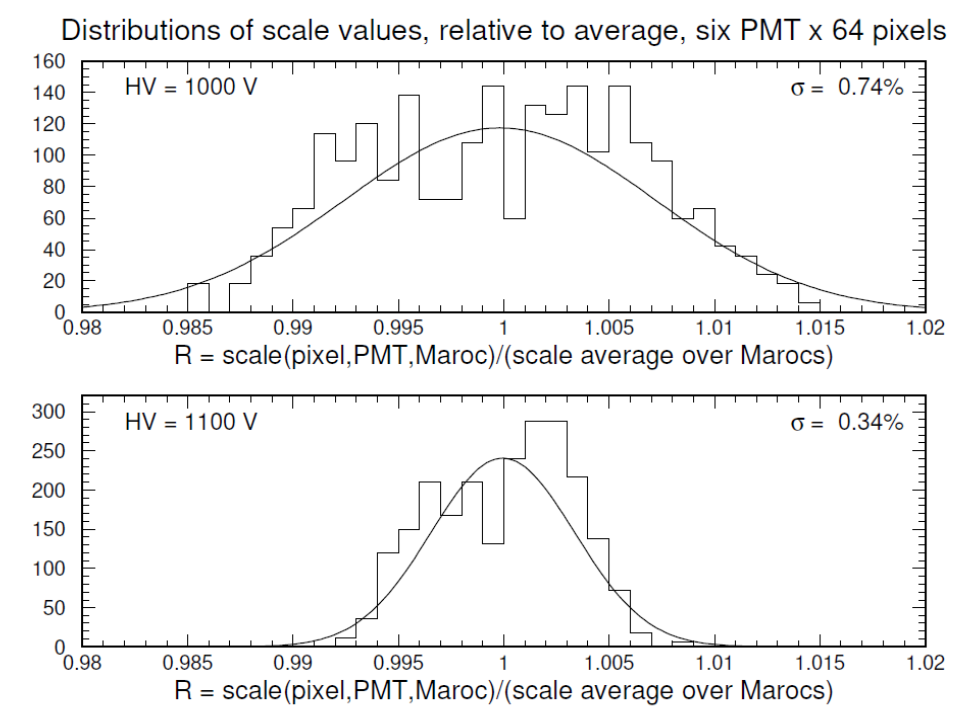
\includegraphics[width=0.98\linewidth, trim=0 10 15 10, clip]{figures/R_scale_maroc_avg.png}
	\caption{Evaluated precision of the scale parameter measurement for the two high voltage settings.}
	\label{fig:R_scale_maroc_avg}
\end{figure}


Fig. \ref{fig:pglobal_qe_all} shows the pattern similar to Fig. \ref{fig:pglobal_sc} for the $\mu$ parameter, with the difference that $\mu$ essentially does not depend on high voltage, but it is proportional to the light intensity. The plot shows that the distributions at different high voltages are on top of each other at a given light intensity, but shift in log scale when light intensity changes. In the plot the parameter $\mu$ is shown normalized to the number of photons coming to each pixel in the ``wheel position 3'' setting, to provide the value of quantum efficiency in it. 
\begin{figure}[hbt]
	\centering
	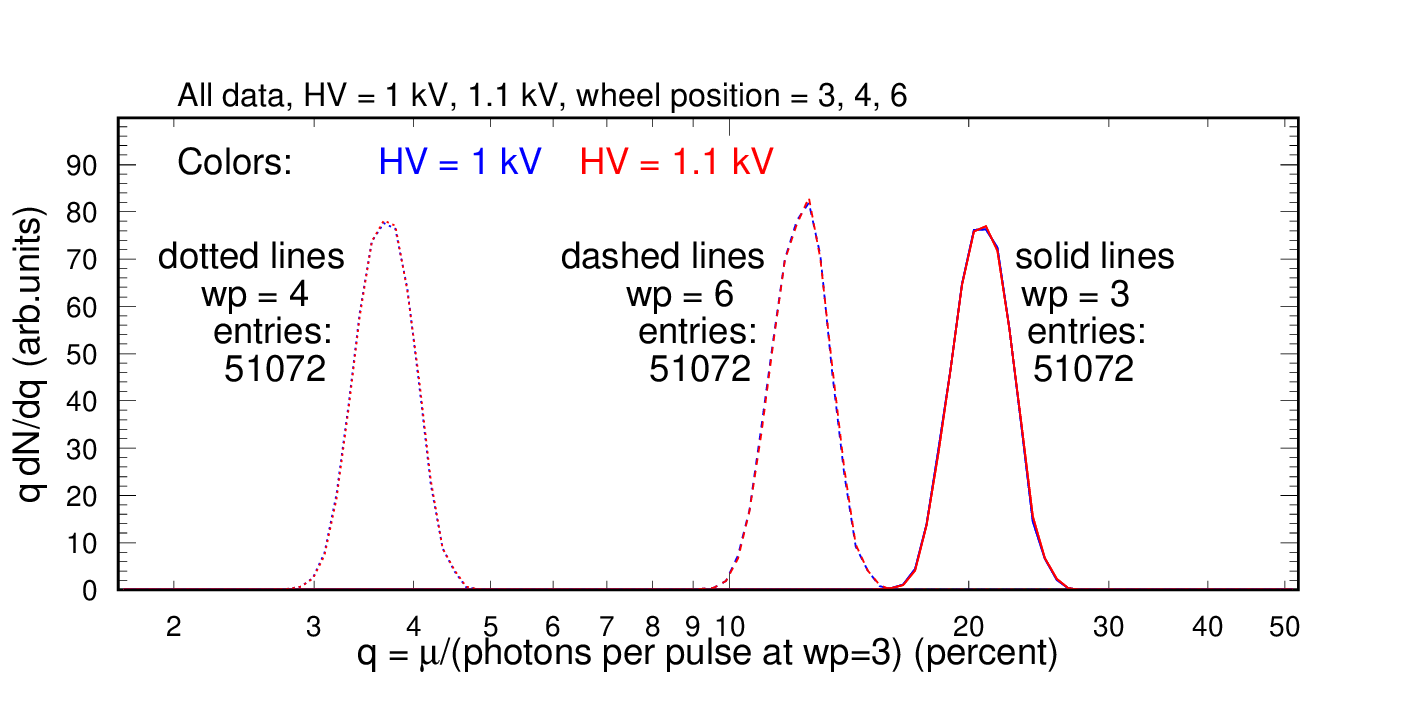
\includegraphics[width=0.98\linewidth,trim=0 15 50 35,clip]{figures/pglobal_qe_all.pdf}
	\caption{Distribution of $\mu$ divided by the measured number of photons per pulse at wheel position 3. All measured pixels contributed to the plots. Distributions measured at HV = 1000 V are shown by violet, the ones at HV = 1100 V by red color (essentially on top of each other). The three line styles (dotted, dashed, and solid) correspond to different illumination. For the data collected at wheel position 3, this ratio is the quantum efficiency of the individual pixels.}
	\label{fig:pglobal_qe_all}
\end{figure}

Fig. \ref{fig:pglobal_mHV} illustrates the stability of the evaluated $\mu$ parameter measured at different values of HV. As we had only two HV settings, the plot shows the distributions of the ratios $R_{\mu\mathrm{HV}} = \mu_{\mathrm{HV1.1}}/\mu_{\mathrm{HV1.0}}$ of the values of $\mu$ measured at 1.1 kV to the values at 1.0 kV. The width of the distribution around the $R = 1$ value may characterize the statistical error in the measurement of $\mu$ parameter. The plot shows that the relative $\mu$ spread is approximately within 1\% of the value. In the first approximation the quantum efficiency is not expected to be dependent on the HV applied to a PMT. However, the distributions show a slight systematic shifts in the distributions of the ratio, indicating to the small dependence of quantum efficiency on the high voltage applied, with a slope of about 0.2\% per 100 V change. Practically the change is insignificant and within the statistical errors, however, there might be some some attempts to explain it assuming, for example, that the larger electric field at the cathode region may improve the probability of photoelectron knock out, or improve the collection probability of the photoelectrons at the first dynodes.
\begin{figure}[hbt]
	\centering
	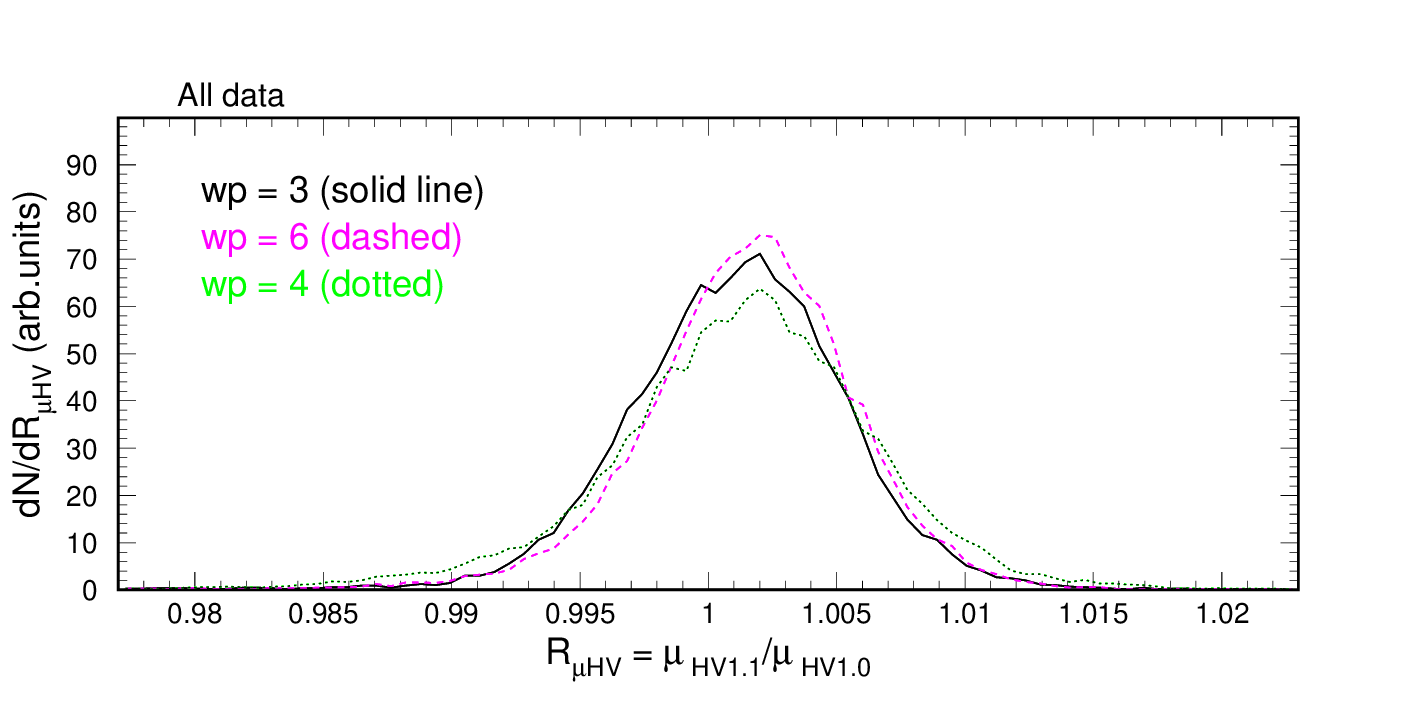
\includegraphics[width=0.98\linewidth, trim=0 15 50 35, clip]{figures/pglobal_mHV.pdf}
	\caption{The ratio of the $\mu$ parameters from the fit results at HV = 1100 V to the results at HV = 1000 V.}
	\label{fig:pglobal_mHV}
\end{figure}

Fig. \ref{fig:pglobal_eff} shows the estimated values of the photodetection efficiency based on the calculated optimal threshold value for the separation of the single photoelectron events from pedestal (including the cross talk background). The calculation for every pixel was performed for the measurements at the lowest illumination settings at the wheel position 4, when both parameters $\mu$ and $\beta$ are small and the probabilities of having two cross talk electrons in one event are negligible. Such condition imitates the real operations of the MAPMTs in the RICH detector in the best way, as the number of photons from one relativistic particle is expected to be small. The figure also illustrates the generally very high (above 96\%) level of the single photon efficiency of all tested H12700 PMTs at the planned operational HV value of 1 kV. The efficiency is improved significantly at HV = 1.1 kV, with the value of "inefficiency" decreasing by approximately a factor of 2 in these conditions.
\begin{figure}[hbt]
	\centering
	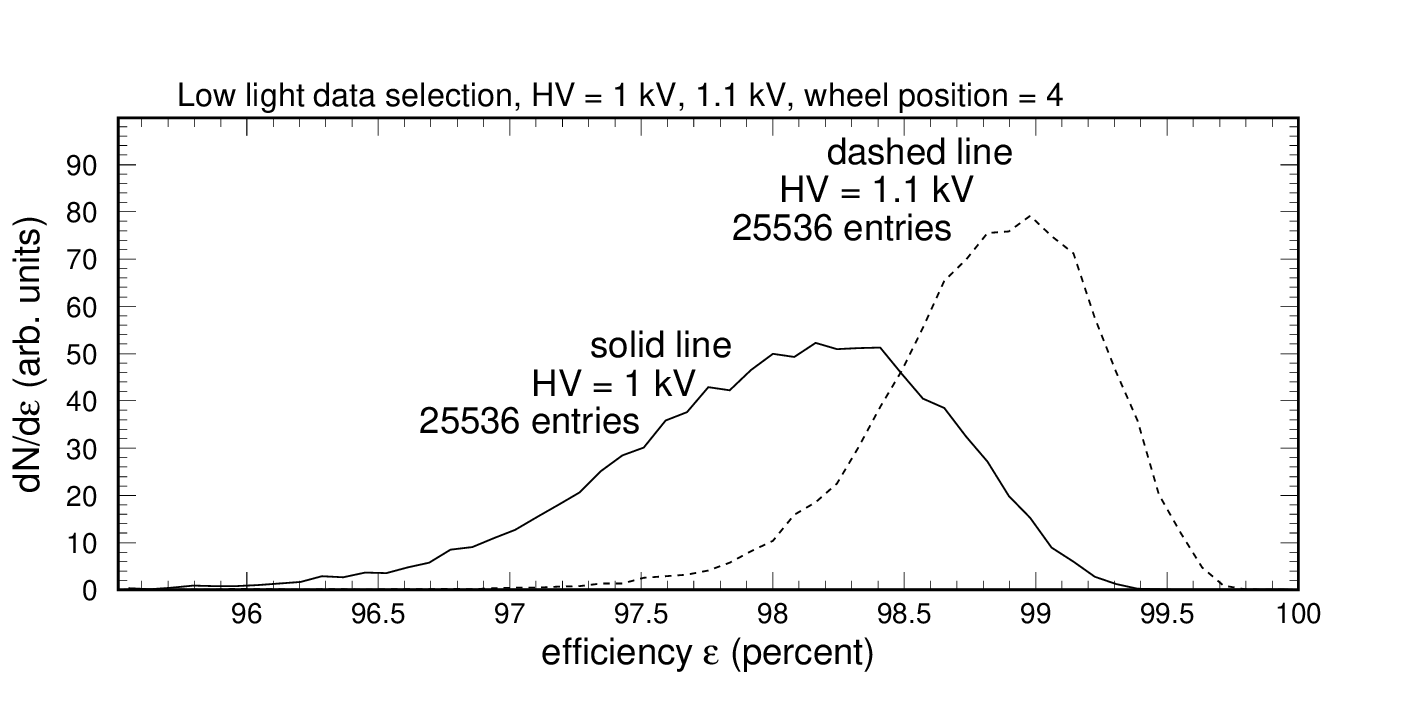
\includegraphics[width=0.98\linewidth, trim=0 15 50 35, clip]{figures/pglobal_eff.pdf}
	\caption{Distribution of the measured efficiency for all pixels at wheel position 4.}
	\label{fig:pglobal_eff}
\end{figure}

The efficiency improvements at larger HV values are correlated with the observed increases of the average degree of multiplication of photoelectrons on the first dynodes of MAPMTs. The average gain $\nu$ is evaluated in the model using the five parameters describing the shapes of the SPE amplitude distributions. The average gain is clearly dependent on the energy acquired by the photoelectron traveling from the photocathode to the first dynode. The spread in this parameter over the whole data set is noticeable, but the systematic increase at HV = 1.1 kV is quite prominent, as shown in Fig. \ref{fig:pglobal_nu}. This figure further illustrates the consistency and stability of the fitting procedure as the distributions built for different illuminating conditions are very close to each other.
\begin{figure}[hbt]
	\centering
	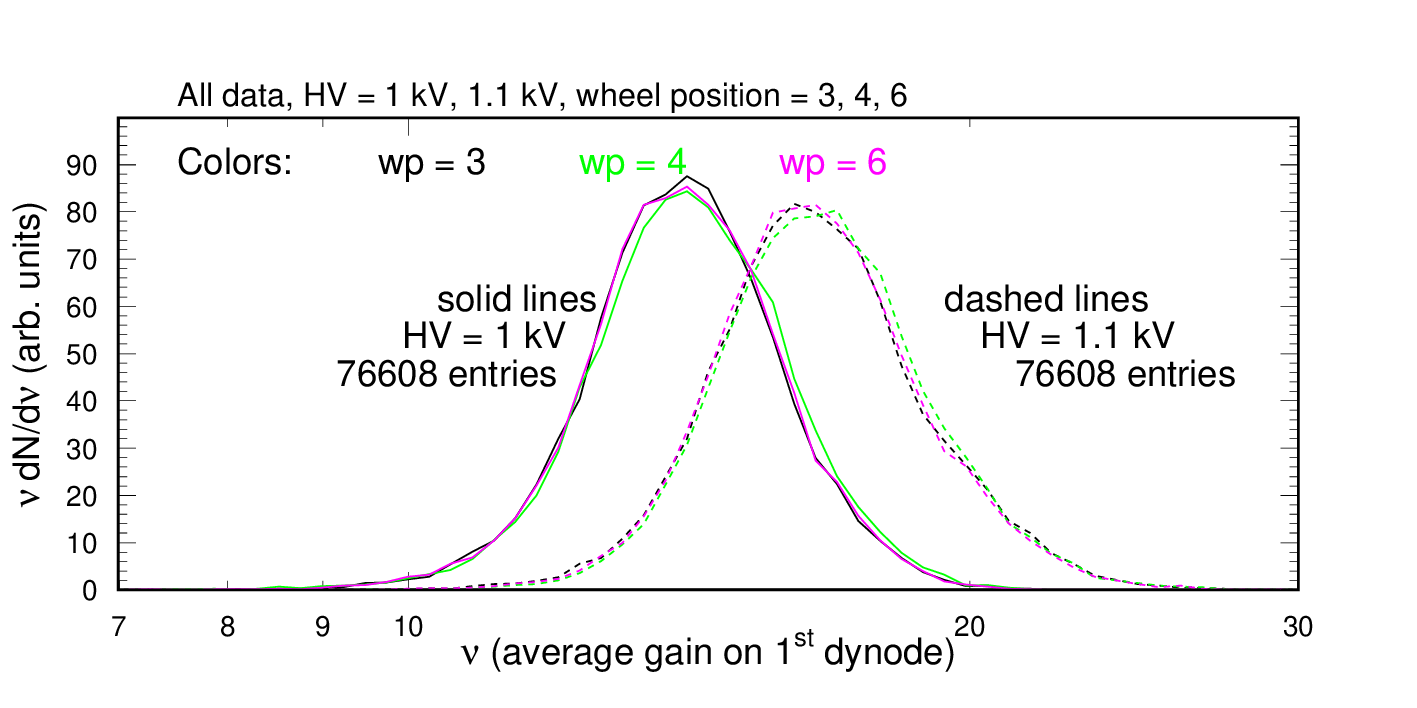
\includegraphics[width=0.98\linewidth, trim=0 15 50 35,clip]{figures/pglobal_nu.pdf}
	\caption{Distribution of $\nu$ (average gain on $1^{\mathrm{st}}$ dynode) as determined by the fitting procedure for a set of 399 PMTs.}
	\label{fig:pglobal_nu}
\end{figure}


Fig. \ref{fig:pglobal_Rn} is similar to Fig. \ref{fig:pglobal_Rs}, showing the measured $\nu$ parameters normalized to the value of $\nu$ averaged over the three measurements on the same pixel at the three different illuminations. The value of the ratio $R_{\mathrm{n}}$ serves as an estimate of the statistical error of the $\nu$ evaluation procedure, and is approximately within 5\%. The distribution is visibly non-Gaussian as $\nu$ is the complicated function of five variable signal shape parameters in the fit. There is a small difference between the distributions at different HV.
\begin{figure}[hbt]
	\centering
	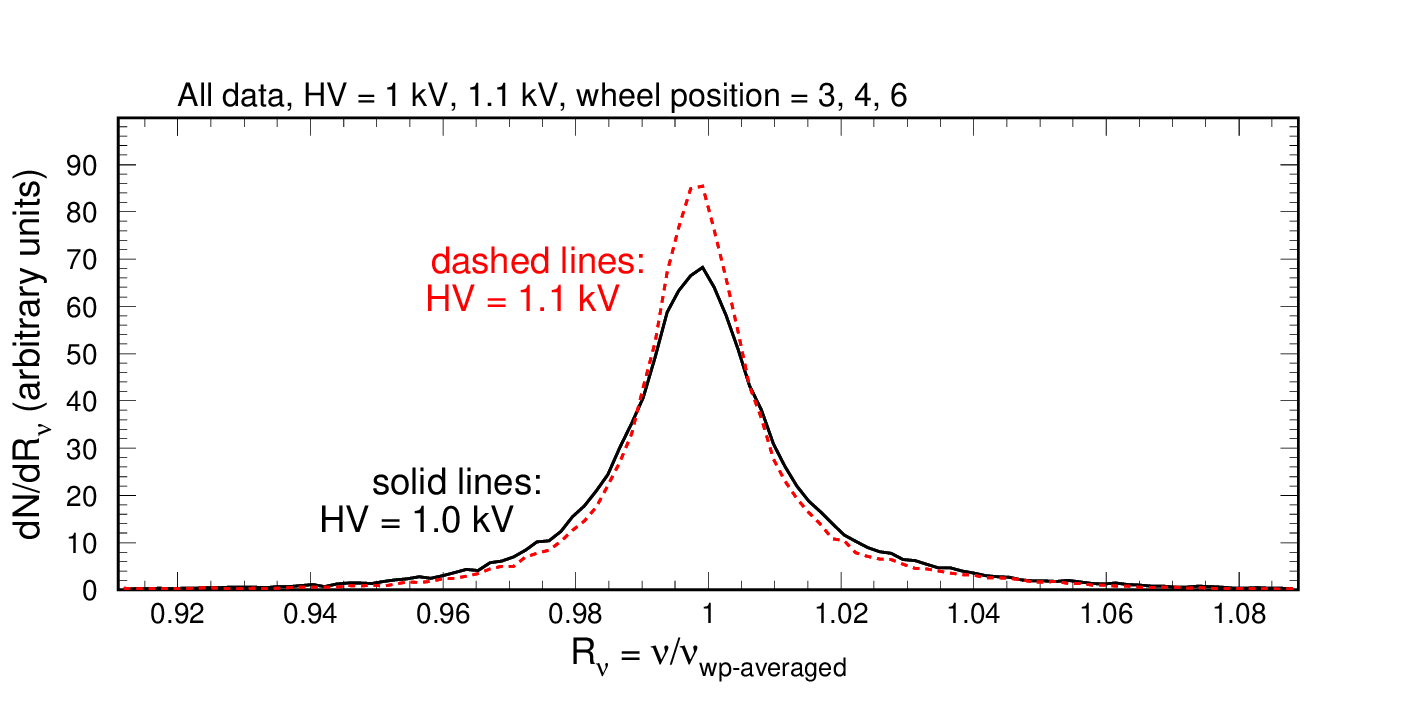
\includegraphics[width=0.98\linewidth, trim=0 15 50 35, clip]{figures/pglobal_Rn.pdf}
	\caption{Parameter $\nu$ normalized to its average value over the three different illumination settings (wheel positions 3, 4, and 6).}
	\label{fig:pglobal_Rn}
\end{figure}


Fig. \ref{fig:2d_avg_fit_results} illustrates the dependencies of several major parameters on the pixel number for the full set of MAPMTs studied, including the average amplitude of the single photon amplitude $scale$, Quantum Efficiency, the relative probability of the cross talk events $\beta/\mu$, and evaluated efficiency. Generally, the set exhibits a very good uniformity of the average parameters, much smaller than the spreads observed between pixels in a single MAPMT, or between the tubes. The Quantum efficiency is slightly higher at the edges of the MAPMT and still higher at the corners (larger areas of the border pixels are taken into account in the QE calculation). The cross talk probability pattern is consistent with the hypothesis that it is dependent on the number of neighbors: it is smaller at the edges, and still smaller in the corners of the MAPMT. The four outliers in pixels# 16, 24, 32, and 40 are most likely due to the feature of all Maroc boards used, exhibiting significantly wider pedestals in these pixels, hiding the cross talk inder the pedestal Gaussian and making the fitting procedure fail to fit the cross talk properly. The average efficiency pattern shows somewhat better values in columns 4 an 8, likely correlated with the widths of the cross talk contributions.    
\begin{figure*}[hbt]
	\centering
	\begin{subfigure}[c]{0.24\linewidth}
		\centering
		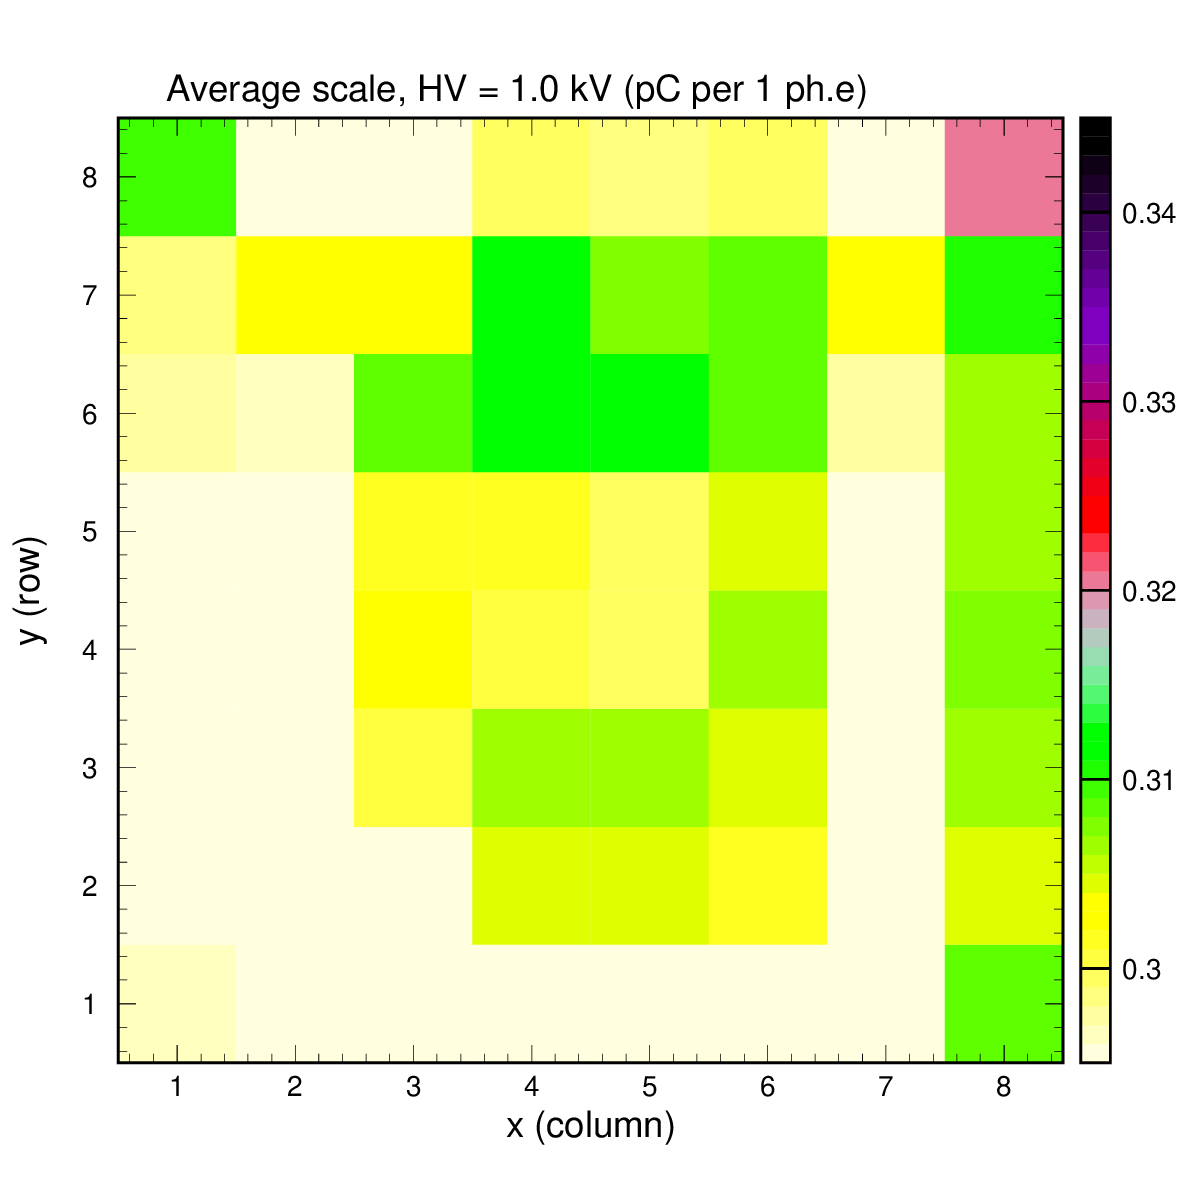
\includegraphics[width=\linewidth, trim={0mm 0mm 0mm 19mm},clip]{figures/pglobal_sc2d.pdf}
		\caption{Scale, HV = 1.0 kV (pC per 1 ph.e)}
		\vspace{0mm}
	\end{subfigure}%%
	\begin{subfigure}[c]{0.24\linewidth}
		\centering
		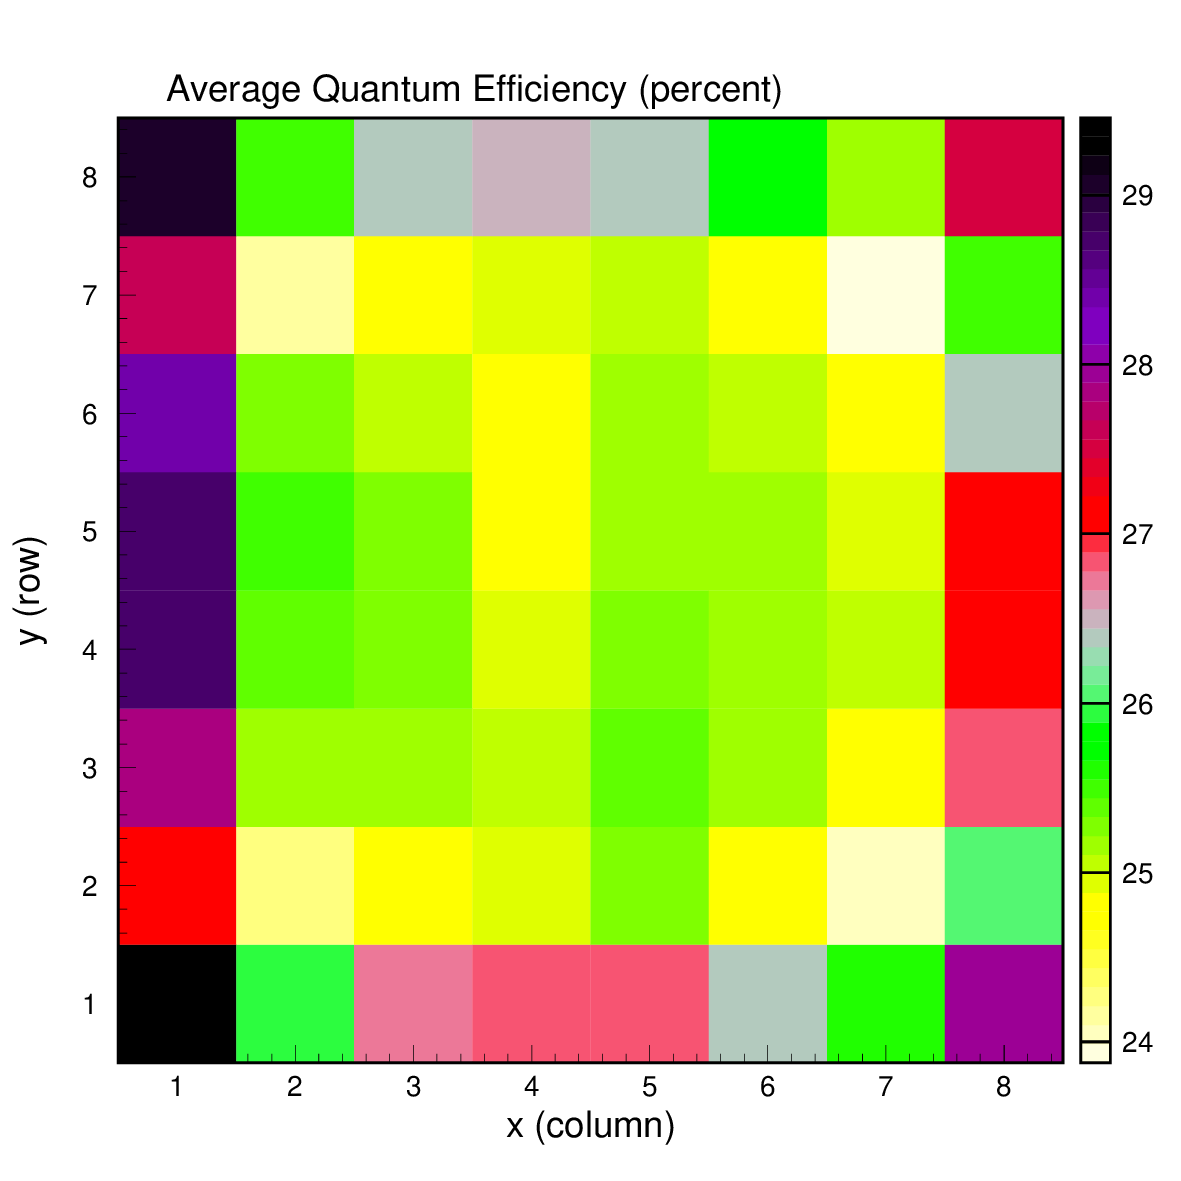
\includegraphics[width=\linewidth, trim={0mm 0mm 0mm 19mm},clip]{figures/pglobal_qe.pdf}
		\caption{Quantum Efficiency (percent)}
		\vspace{0mm}
	\end{subfigure}%%
	\vspace{3mm}
	\begin{subfigure}[c]{0.24\linewidth}
		\centering
		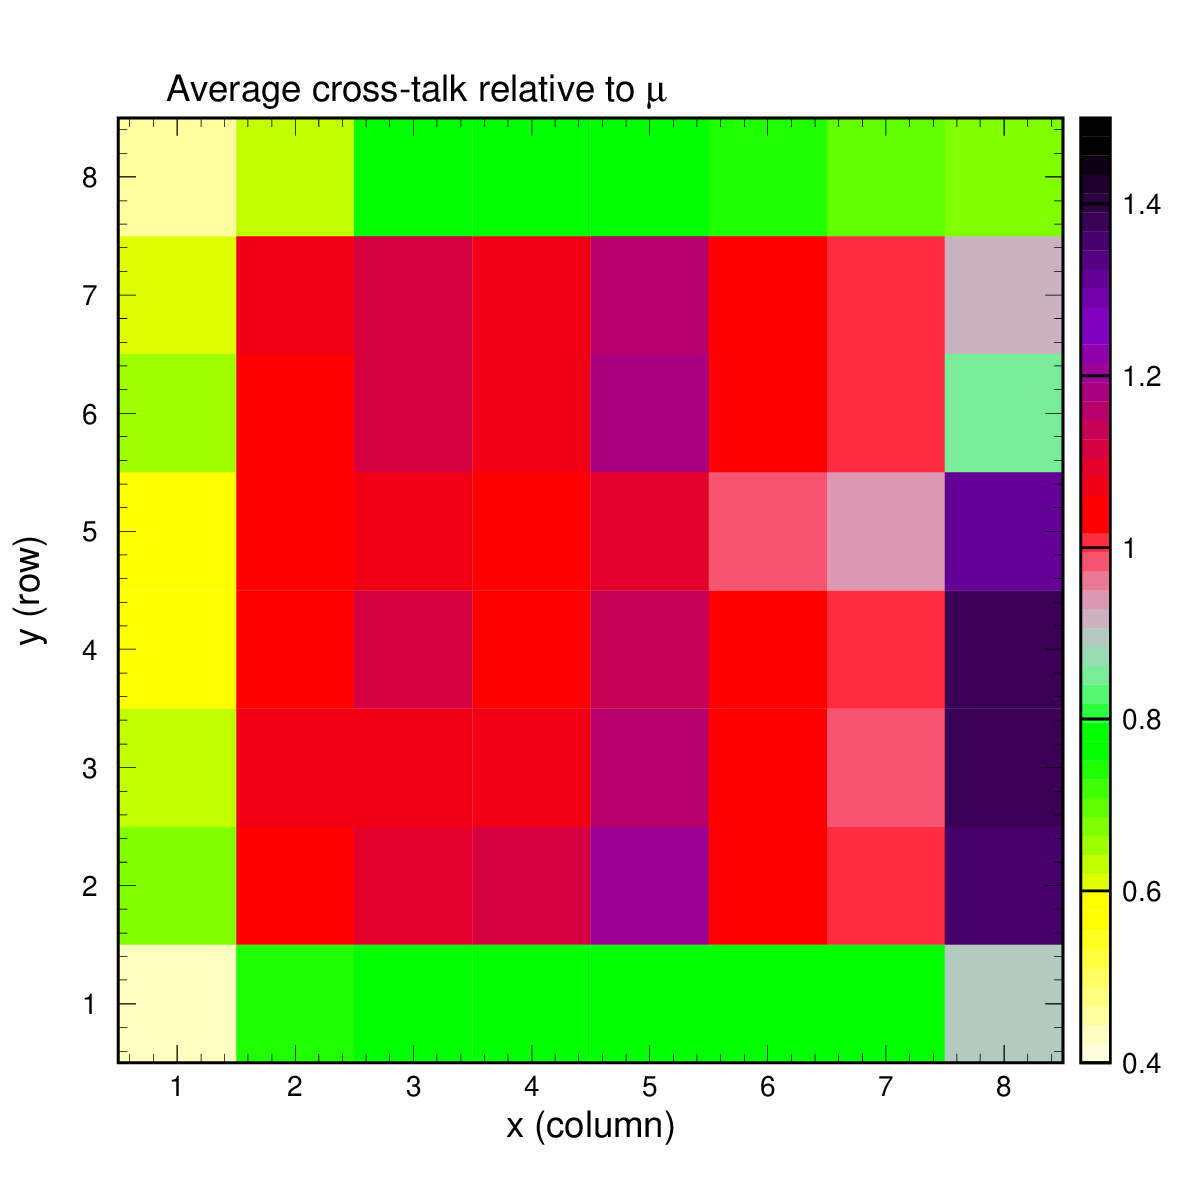
\includegraphics[width=\linewidth, trim={0mm 0mm 0mm 19mm},clip]{figures/pglobal_beta.pdf}
		\caption{Cross-talk relative to $\mu$}
		\vspace{0mm}
	\end{subfigure}%%
	\begin{subfigure}[c]{0.24\linewidth}
		\centering
		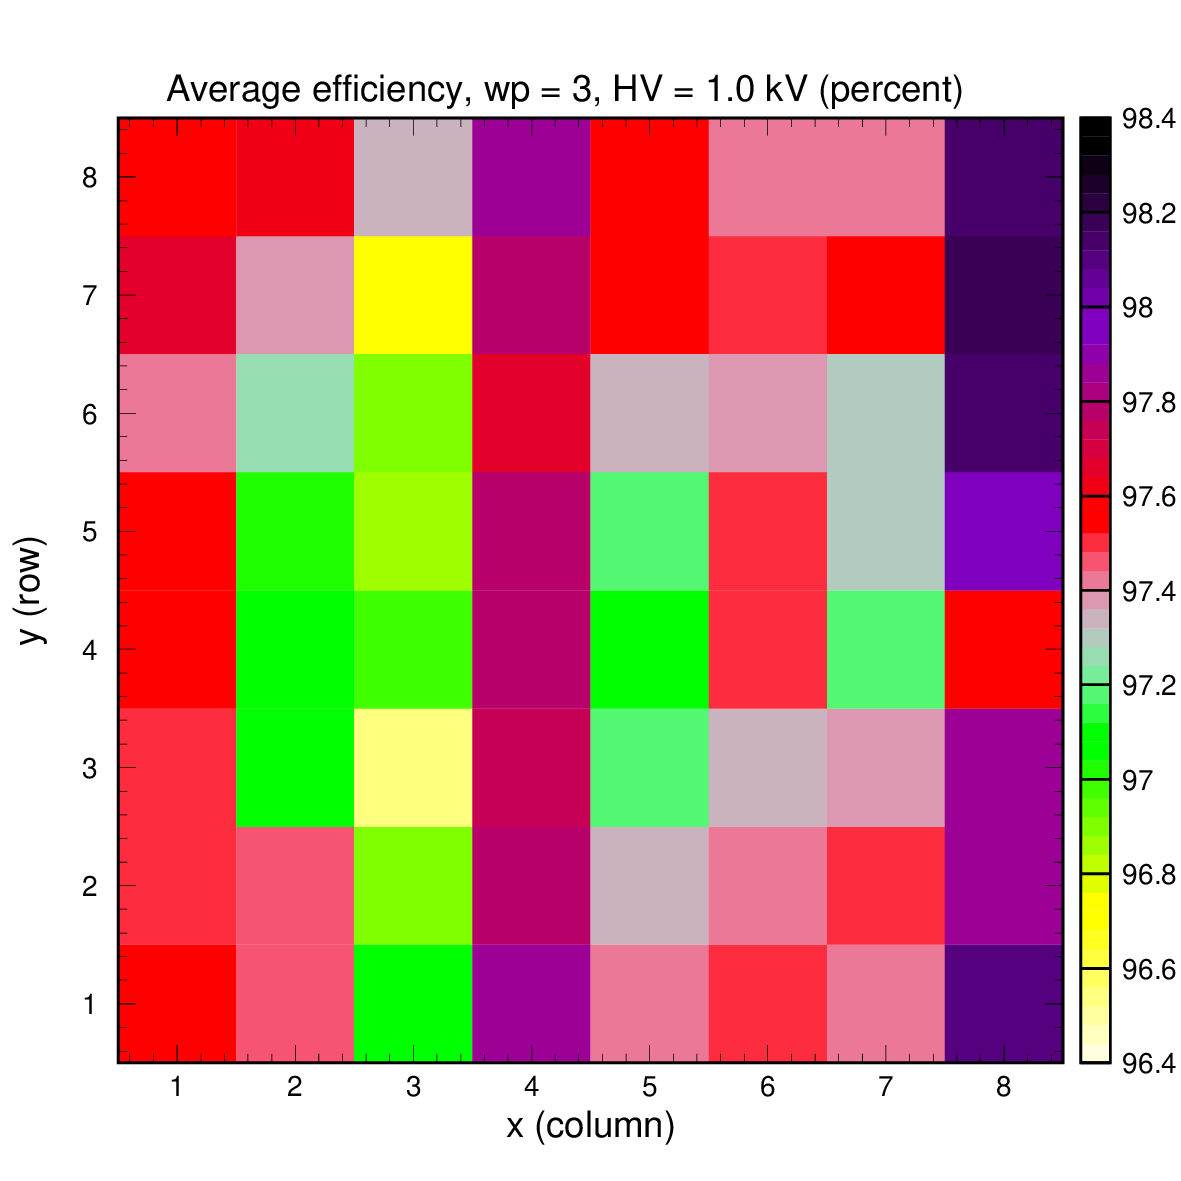
\includegraphics[width=\linewidth, trim={0mm 0mm 0mm 19mm},clip]{figures/pglobal_eff2d.pdf}
		\caption{Efficiency, wp = 3, HV = 1.0 kV (percent)}
		\vspace{0mm}
	\end{subfigure}%%
	\caption{Two dimensional plots showing the average (a) scale, (b) quantum efficiency, (c) cross-talk relative to $\mu$, (d) cross-talk relative to scale, and (e) efficiency as a function of pixel location. The results are averaged for the full set of 399 MAPMTs Hamamatsu H12700}
	\label{fig:2d_avg_fit_results}
\end{figure*}



The parameter database accumulated as the result of this work was used for the selection of the MAPMTs for installation in the RICH detector, and for the optimization of the future run parameters, such as the tube placement selection, setting the values of operating high voltage, electronics gains and thresholds in the detector.


The data also provide the opportunity to evaluate the spread of such parameters in the mass production of the MAPMT devices as the channel gains, quantum efficiencies, SPE spectral shapes, parameters of the cross-talk, - across the face of each tube, and across the whole set. The results show that the quality of MAPMT mass production at Hamamatsu is high and satisfies our needs in the good quality single photoelectron detection.



%We saw that although there is little difference in crosstalk signals, the H12700 PMTs suffer less from dark current, have narrower SPE spectra, and have higher $\mu$ and relative efficiency values.
%An example plot of the $\mu$'s and relative efficiencies of H8500 and H12700 PMTs with similar low and high gains is shown in Figure \ref{efficiency}.

%We see that the relative efficiency is closely related to the $\mu$ which is on average, over all pixels at all voltages for all the PMTs we tested, $29\pm5$ percent higher in H12700 than H8500 MAPMTs. One concern with these $\mu$ measurements however is that the laser system used to measure these PMTs was only incident on a portion of each pixel, consequently missing their sum total effect and pinpointing possible spatial dependencies which should be further studied and perhaps remeasured with a fully illuminated MAPMT instead of collimated pinpoint laser light. In terms of crosstalk for the two varieties of MAPMT the H12700s appear to be better than the H8500s. The H12700s have a decrease in crosstalk by nearly a factor of two. Additional studies of dark current in the H12700s would be useful, as the dark current is usually dominated by individual pixels or bad regions of the PMT instead of spread around evenly like in the H8500s, but overall the two varieties are not very different in terms of dark current.